\documentclass[10pt, xetex, hyperref={pdfpagelabels=false}]{beamer}

% -------------------------------------------------------------------
% Packages
% -------------------------------------------------------------------
\usepackage[english]{babel}
\usepackage{amsmath, amsthm, amssymb}

% -------------------------------------------------------------------
% Natural deduction proofs
% -------------------------------------------------------------------
\usepackage{bussproofs}
\EnableBpAbbreviations
\def\extraVskip{3pt}

% https://tex.stackexchange.com/questions/104554/
% how-to-scale-prooftree-environment-bussproofs-package
\newenvironment{scprooftree}[1]%
  {\gdef\scalefactor{#1}\begin{center}\proofSkipAmount \leavevmode}%
  {\scalebox{\scalefactor}{\DisplayProof}\proofSkipAmount \end{center} }

% -------------------------------------------------------------------
% -- Algorithms
% -------------------------------------------------------------------

\usepackage{algorithm,algpseudocode}
% -------------------------------------------------------------------

\usepackage{fancyvrb}
\usepackage{geometry}
\usepackage{graphicx}
\usepackage{lmodern}
\usepackage{url}

% --------------------------------------------------------------------------
% Color definitions.
% --------------------------------------------------------------------------
\usepackage{xcolor}
\definecolor{blu}{RGB}{1,0,102}
\definecolor{decoration}{RGB}{10,164,216}
\definecolor{darkred}{rgb}{0.5, 0.0, 0.13}
\definecolor{darkgreen}{rgb}{0.0, 0.5, 0.0}

% --------------------------------------------------------------------------
% Beamer configuration.
% --------------------------------------------------------------------------
\usetheme{default}
\usecolortheme{default}
% \usefonttheme{serif}

\beamertemplatenavigationsymbolsempty
\setbeamertemplate{navigation symbols}{}
\hypersetup{pdfpagemode=UseNone}

% footer.
\setbeamercolor{headFoot}{fg=gray, bg=white}

\setbeamertemplate{footline}{
  \leavevmode%
  \hbox{%
  % \begin{beamercolorbox}
  %   [wd=.8\paperwidth,ht=2.3ex,dp=1ex,left]{headFoot}%
  %   \hspace*{2ex}\textbf\insertshorttitle\hspace*{2mm}|
  %   \hspace*{2mm}\textbf\insertshortauthor
  % \end{beamercolorbox}%
  \begin{beamercolorbox}
    [wd=\paperwidth,ht=2.4ex,dp=1ex,right]{headFoot}%
    \insertframenumber{}/\inserttotalframenumber\hspace*{2ex}
  \end{beamercolorbox}}%
  \vskip 0pt%
}

\setbeamerfont{frametitle}{series=\bfseries}
\setbeamercolor{frametitle}{fg=white,bg=blu}

\setbeamerfont{framesubtitle}{size=\normalfont\scriptsize}
\setbeamercolor{framesubtitle}{fg=white, bg=blu}

\setbeamercolor{background canvas}{bg=white}
\setbeamercolor{normal text}{fg=black}

% \setbeamercolor{institute}{fg=blu}
\setbeamercolor{title}{fg=blu}
% \setbeamercolor{subtitle}{fg=blu}

% \setbeamercolor{titlelike}{fg=blu}
\setbeamerfont{footnote}{size=\tiny}
\setbeamercolor{footnote}{fg=gray}
% \setbeamercolor{block title}{bg=blu,fg=blu}
% \setbeamercolor{block body}{bg=aliceblue}
% \setbeamercolor{item}{fg=blu} % color of bullets
% \setbeamercolor{subitem}{fg=blu}
% \setbeamercolor{itemize/enumerate subbody}{fg=blu}
% \setbeamertemplate{itemize subitem}{{\textendash}}
% \setbeamerfont{itemize/enumerate subbody}{size=\footnotesize}
% \setbeamerfont{itemize/enumerate subitem}{size=\footnotesize}

% --------------------------------------------------------------------------
% Fonts
% --------------------------------------------------------------------------
\usefonttheme{professionalfonts}
% \usefonttheme{serif}

\usepackage{fontspec}
\usepackage{mathtools}
\usepackage{unicode-math}

% \newfontfamily\djvu[ExternalLocation=fonts/
%   , BoldFont=DejaVuSansMono-Bold.ttf
%   , BoldItalicFont=DejaVuSansMono-BoldOblique.ttf
%   , ItalicFont=DejaVuSansMono-Oblique.ttf
%   ]{DejaVuSansMono.ttf}

% \setmonofont[ExternalLocation=fonts/
% , BoldFont=DejaVuSansMono-Bold.ttf
% , BoldItalicFont=DejaVuSansMono-BoldOblique.ttf
% , ItalicFont=DejaVuSansMono-Oblique.ttf
% ]{DejaVuSansMono.ttf}

% \setmathfont[ExternalLocation=fonts/
%   ]{DejaVuMathTeXGyre.ttf}
% \newfontfamily\mathfont{fonts/DejaVuMathTeXGyre.ttf}


% \newfontfamily\sourcecode[ExternalLocation=fonts/
%   , BoldFont=SourceCodePro-Semibold.ttf
%   , BoldItalicFont=SourceCodePro-SemiboldIt.ttf
%   , ItalicFont=SourceCodePro-It.ttf
%   ]{SourceCodePro-Regular.ttf}

% -------------------------------------------------------------------
% Tikz Configuration
% -------------------------------------------------------------------

\usepackage{tikz}
\usetikzlibrary{positioning}
\usetikzlibrary{arrows}
\usetikzlibrary{calc}
\usetikzlibrary{shapes}
\usepackage{rotating}

\tikzset{
  hyperlink node/.style={
    alias=sourcenode,
    append after command={
        let     \p1 = (sourcenode.north west),
            \p2=(sourcenode.south east),
            \n1={\x2-\x1},
            \n2={\y1-\y2} in
        node [inner sep=0pt, outer sep=0pt,anchor=north west,at=(\p1)]
        {\hyperlink{#1}{\XeTeXLinkBox{\phantom{\rule{\n1}{\n2}}}}}
                %xelatex needs \XeTeXLinkBox, won't create a link unless it
                %finds text --- rules don't work without \XeTeXLinkBox.
                %Still builds correctly with pdflatex and lualatex
    }
  }
}

\tikzstyle{vertex}=[
    auto=left
  , circle
  , fill=black!25
  , minimum size=5pt
  , inner sep=0pt
  ]

% -------------------------------------------------------------------
% Listings
% -------------------------------------------------------------------

\usepackage{listings}
\usepackage{lstautogobble}

\lstdefinestyle{TPTP}{
    aboveskip=10pt
  , basicstyle=\tt
  , belowskip=10pt
  , keywords=[2]{axiom
    , conjecture
    , inference
    , negated_conjecture
    , plain
    , source}
  , keywords=[3]{fof, cnf}
  , keywords=[4]{canonicalize, resolve, conjunct,
    strip, simplify, negate, clausify}
  , keywordstyle=[2]\bfseries
  , keywordstyle=[3]\bfseries
  , keywordstyle=[4]\bfseries
  , showstringspaces=false
  , keepspaces=true
}

\lstnewenvironment{tptp}
  {\lstset{style=TPTP,columns=fullflexible}\csname lst@SetFirstLabel\endcsname}
  {\csname lst@SaveFirstLabel\endcsname}

% \usepackage{autofe}
% \usepackage{afterpage}
% \usepackage{comment}
% \usepackage[hyphens]{url}
% \usepackage{bm}

\usepackage{amssymb}
\usepackage{amsmath}

\let\proof\relax      %% https://tex.stackexchange.com/questions/43835/
\let\endproof\relax   %% conflict-between-amsthm-and-some-other-package
\usepackage{amsthm}

\newenvironment{sketchproof}{%
  \renewcommand{\proofname}{Sketch of the Proof}\proof}{\endproof}

\renewcommand\qedsymbol{$\blacksquare$}

%\usepackage{stmaryrd} %new symbol font for tcs
% \usepackage{color}
\usepackage{fancybox}
% \usepackage{minted}
% \setminted[cagda]{
%   bgcolor   = aliceblue
% , fontsize  = \footnotesize
% , frame     = none
% % , framerule = 0.4pt
% % , framesep  = 0pt
% , style     = cagda
% }

% -------------------------------------------------------------------
% Verbatim.
% -------------------------------------------------------------------

\usepackage{verbatim}
\usepackage{relsize}
\usepackage{fancyvrb}
% \DefineVerbatimEnvironment
%   {code}{Verbatim}
%   { fontsize=\relsize{-2}
%   , fontfamily=freemodo
%   , frame =single
%   , framesep=5mm
%   , showspaces=true
%   , obeytabs=true
%   } % {}

\setcounter{secnumdepth}{5}

\renewcommand*\rmdefault{cmr}

% -------------------------------------------------------------------
% New commands
% -------------------------------------------------------------------

\usepackage{textcomp}
\usepackage[verbose]{newunicodechar}

\newunicodechar{¬}{\ensuremath{\neg}\;}
\newunicodechar{Γ}{\ensuremath{\Gamma}}
\newunicodechar{γ}{\ensuremath{\gamma}}
\newunicodechar{φ}{\ensuremath{\varphi}}
\newunicodechar{ψ}{\ensuremath{\psi}}
\newunicodechar{ϕ}{\ensuremath{\varphi}}
\newunicodechar{ᵢ}{\ensuremath{{}_{i}}}
\newunicodechar{₀}{\ensuremath{{}_{0}}}
\newunicodechar{₁}{\ensuremath{{}_{1}}}
\newunicodechar{₂}{\ensuremath{{}_{2}}}
\newunicodechar{₃}{\ensuremath{{}_{3}}}
\newunicodechar{₄}{\ensuremath{{}_{4}}}
\newunicodechar{₅}{\ensuremath{{}_{5}}}
\newunicodechar{₆}{\ensuremath{{}_{6}}}
\newunicodechar{₇}{\ensuremath{{}_{7}}}
\newunicodechar{₈}{\ensuremath{{}_{8}}}
\newunicodechar{₉}{\ensuremath{{}_{9}}}
\newunicodechar{ₙ}{\ensuremath{{}_{n}}}
\newunicodechar{ₘ}{\ensuremath{{}_{m}}}
\newunicodechar{ℓ}{\ensuremath{\ell}}
\newunicodechar{→}{\ensuremath{\rightarrow}}
\newunicodechar{⇒}{\ensuremath{\Rightarrow}}
\newunicodechar{⇔}{\ensuremath{\Leftrightarrow}}
\newunicodechar{∅}{\ensuremath{\emptyset}}
\newunicodechar{∈}{\ensuremath{\in}}
\newunicodechar{∘}{\ensuremath{\circ}}
\newunicodechar{∙}{\ensuremath{\bullet}}
\newunicodechar{∧}{\ensuremath{\wedge}}
\newunicodechar{∨}{\ensuremath{\vee}}
\newunicodechar{∼}{\ensuremath{\sim}}
\newunicodechar{≠}{\ensuremath{\neq}}
\newunicodechar{≡}{\ensuremath{\equiv}}
\newunicodechar{⊕}{\ensuremath{\oplus}}
\newunicodechar{⊖}{\ensuremath{\ominus}}
\newunicodechar{⊢}{\ensuremath{⊢}}
\newunicodechar{⊤}{\ensuremath{\top}}
\newunicodechar{⊥}{\ensuremath{\bot}}
\newunicodechar{⊻}{\ensuremath{\veebar}}
\newunicodechar{⟝}{\ensuremath{⊢}}
\newunicodechar{⬓}{\ensuremath{\square}}
\newunicodechar{ⱼ}{\ensuremath{{}_{j}}}
\newunicodechar{λ}{\ensuremath{\lambda}}

\usepackage{xspace}

\newcommand{\abbre}[1]{\textsc{#1}\xspace}
\newcommand{\ATPs}{\abbre{ATPs}}
\newcommand{\ATP}{\abbre{ATP}}
\newcommand{\Bool}{\abbre{Bool}}
\newcommand{\CNF}{\abbre{CNF}}
\newcommand{\CPL}{\abbre{CPL}}
\newcommand{\ITP}{\abbre{ITP}}
\newcommand{\ITPs}{\abbre{ITPs}}
\newcommand{\List}{\abbre{List}}
\newcommand{\NProp}{\abbre{Prop}}
\newcommand{\Nat}{\abbre{Nat}}
\newcommand{\Prop}{\abbre{Prop}}
\newcommand{\Source}{\abbre{Premise}}
\newcommand{\Target}{\abbre{Conclusion}}
\newcommand{\Lit}{\abbre{Lit}}
\newcommand{\SAT}{\abbre{SAT}}
\newcommand{\SMT}{\abbre{SMT}}

\newcommand{\name}[1]{\texttt{#1}\xspace}
\newcommand{\canonicalize}{\name{canonicalize}}
\newcommand{\clausify}{\name{clausify}}
\newcommand{\conjunct}{\name{conjunct}}
\newcommand{\negate}{\name{negate}}
\newcommand{\resolve}{\name{resolve}}
\newcommand{\simplify}{\name{simplify}}
\newcommand{\strip}{\name{strip}}
\newcommand{\tptpaxiom}{\name{axiom}}
\newcommand{\tptpconjecture}{\name{conjecture}}

\newcommand{\nnf}{\name{nnf}}

\newcommand{\prg}[1]{\texttt{#1}\xspace}
\newcommand{\Agda}{\prg{Agda}}
\newcommand{\Athena}{\prg{Athena}}
\newcommand{\IsabelleHOL}{\prg{IsabelleHOL}}
\newcommand{\Metis}{\prg{Metis}}

\newcommand{\len}[1]{\texttt{#1}\xspace}
\newcommand{\Haskell}{\len{Haskell}}
\newcommand{\TPTP}{\len{TPTP}}
\newcommand{\TSTP}{\len{TSTP}}

\newcommand{\NN}{\ensuremath{\mathbb{N}}}

\newcommand{\fun}[1]{ {\fontseries{sb}\selectfont \textsf{#1}} \xspace}

\newcommand{\zero}{\fun{zero}}
\newcommand{\suc}{\fun{succ}}
\newcommand{\fassoc}{\fun{assoc}}
\newcommand{\fbuild}{\fun{build}}
\newcommand{\fcanonicalize}{\fun{canonicalize}}
\newcommand{\fcanon}{\fun{simplify}}
\newcommand{\fclausify}{\fun{clausify}}
\newcommand{\fcnf}{\fun{cnf}}
\newcommand{\fconjunctor}{\fun{disj}}
\newcommand{\fconjunct}{\fun{conjunct}}
\newcommand{\fdist}{\fun{dist}}
\newcommand{\ffactor}{\fun{factor}}
\newcommand{\fform}{\fun{form}}
\newcommand{\fmax}{\fun{max}}
\newcommand{\fndisj}{\fun{ndisj}}
\newcommand{\fnegate}{\fun{negate}}
\newcommand{\fnnfp}{\fun{nnf}₀}
\newcommand{\fnnf}{\fun{nnf}}
\newcommand{\fpolarity}{\fun{polarity}}
\newcommand{\frank}{\fun{rank}}
\newcommand{\frconj}{\fun{rconj}}
\newcommand{\frdisj}{\fun{rdisj}}
\newcommand{\freorder}{\fun{reorder}}
\newcommand{\fresolve}{\fun{resolve}}
\newcommand{\frm}{\fun{rm}}
\newcommand{\frsol}{\fun{rsol}}
\newcommand{\fsbuild}{\fun{sbuild}}
\newcommand{\fsimplify}{\fun{simplify}}
\newcommand{\fstripp}{\fun{strip}\prime}
\newcommand{\fstrip}{\fun{strip}}
\newcommand{\fsubst}{\fun{subst}}
\newcommand{\fuh}{\fun{uh}}

% latin etc. abbrev
\newcommand{\abbrev}[1]{#1} % alternative: \emph{#1}
\newcommand{\cf}{\abbrev{cf.}\ }
\newcommand{\eg}{\abbrev{e.\,g.}}
\newcommand{\Eg}{\abbrev{E.\,g.}}
\newcommand{\ie}{\abbrev{i.\,e.}}
\newcommand{\Ie}{\abbrev{I.\,e.}}
\newcommand{\etal}{\abbrev{et.\,al.}}
\newcommand{\wwlog}{w.\,l.\,o.\,g.} % \wlog is ``write into log file''
\newcommand{\Wlog}{W.\,l.\,o.\,g.}
\newcommand{\wrt}{w.\,r.\,t.}
\newcommand{\TheEnd}{\\\hspace*{0.975\textwidth}$\blacksquare$}

% -------------------------------------------------------------------
% biblatex.
% -------------------------------------------------------------------

\usepackage[%
backend=biber,
backref=true,%
% bibstyle=authoryear,%
% citestyle=authoryear-comp,%
% giveninits=false,%%
isbn=false,%
maxbibnames=6,%
% maxcitenames=4,%
]{biblatex}
\usepackage{csquotes}

\addbibresource{ref.bib}

% Remove the quotes from the title.
\DeclareFieldFormat
  [article,%
  incollection,%
  inproceedings,%
  thesis,% works for mastersthesis and phdthesis
  unpublished,%
  ]{title}{#1}

% Remove "In:" before journal names.
%
% From
% http://tex.stackexchange.com/questions/10682/suppress-in-biblatex
\renewbibmacro{in:}{%
  \ifentrytype{article}{}{\printtext{\bibstring{in}\intitlepunct}}}

% Remove italics from journal names.
\DeclareFieldFormat{journaltitle}{#1}

% Remove italics from proceedings names in articles in proceedings.
\DeclareFieldFormat%
  [incollection,%
  inproceedings,%
  ]{booktitle}{#1}

% Remove italics from the title names.
\DeclareFieldFormat%
 [book,%
 misc,%
 online,%
 report,%
 ]{title}{#1}

% Remove URL if there is DOI.
%
% From:
% https://tex.stackexchange.com/questions/154864/biblatex-use-doi-only-if-there-is-no-url

\renewbibmacro*{doi+eprint+url}{%
  \iftoggle{bbx:url}
    {\iffieldundef{doi}{\usebibmacro{url+urldate}}{}}
    {}%
  \newunit\newblock
  \iftoggle{bbx:eprint}
    {\usebibmacro{eprint}}
    {}%
  \newunit\newblock
    \iftoggle{bbx:doi}
    {\printfield{doi}}
    {}}

\usepackage{silence}
\WarningFilter{biblatex}{Patching footnotes failed}
\WarningFilter{hyperref}{Token not allowed in a PDF string}

% --------------------------------------------------------------------------
% Title and Author
% --------------------------------------------------------------------------

\title[Reconstructing Propositional Proofs in Type Theory]
  {\textbf{Reconstructing Propositional Proofs in Type Theory}}
\date{\today}
\author[Jonathan Prieto-Cubides]{Jonathan Prieto-Cubides\\
Advisor: Andr\'es Sicard-Ram\'irez
}
\institute{
Master in Applied Mathematics\\
Universidad EAFIT\\
Medell\'in, Colombia}
% --------------------------------------------------------------------------

\newsavebox\agdapragma

\begin{document}
\setcounter{page}{1}

% --------------------------------------------------------------------

\begin{frame}[plain]
\titlepage
  \begin{tikzpicture}[overlay, remember picture]
   \tikzset{shift={(current page.center)}}
    \node[xshift=0cm,yshift=-3.2cm] (eafit)
      {
\includegraphics[width=0.2\textwidth]{figures/eafit}};
  \end{tikzpicture}
\end{frame}

% --------------------------------------------------------------------

\begin{frame}{Research}

\begin{block}{Goal}
Formalization in type theory of the classical propositional
derivations generated by the \Metis theorem prover
\end{block}
\pause
\begin{block}{Topics}
\begin{itemize}
\item Automatic reasoning using automatic theorem provers (\ATPs) (\eg, \Metis, \name{EProver})
\item Interactive proving using Proof-assistants (\eg, \Agda, \name{Coq})
\item Formal methods to verify outputs of \ATPs in Proof-assistants
\end{itemize}
\end{block}
\end{frame}

\begin{frame}{Related Work}
In type theory:
\begin{itemize}
  \item \citeauthor{Kanso2012} in \cite{Kanso2012} reconstructs in \Agda propositional proofs generated by \name{EProver} and \name{Z3}
  \item \citeauthor{foster2011integrating} in \cite{foster2011integrating}
  describe proof-reconstruction in \Agda for equational logic of \name{Waldmeister} prover
  \item \citeauthor{Bezem2002} in \cite{Bezem2002} transform a proof produced by the first-order prover \name{Bliksem} in a \name{Coq} proof-term
\end{itemize}
In classical logic:
\begin{itemize}
\item \citeauthor{paulson2007source} in \cite{paulson2007source} introduce
\name{SledgeHammer}, a tool ables to reconstructs proofs of well-known \ATPs: \name{EProver}, \name{Vampire}, among others using \name{SystemOnTPTP} server
\item \citeauthor{Hurd1999} in \cite{Hurd1999} integrates the first-order resolution prover \name{Gandalf} prover for \name{HOL} proof-assistant
\item \citeauthor{kaliszyk2013} in \cite{kaliszyk2013} reconstruct proofs
of different \ATPs for \name{HOL Light}
\end{itemize}
\end{frame}


\begin{frame}[fragile]{Proof Reconstruction: Overview}
\vfill
\begin{center}
\scalebox{0.9}{
\tikzstyle{line} = [draw, -latex']
\begin{tikzpicture}[
   auto
 % , scale=0.15
 , font=\small
 , base/.style =
      { align=center
      }
 , file/.style =
      { base
      , minimum height=3em
      , shape=rectangle
      % , rounded corners
%      , fill=blue!2
      , inner sep=3pt
      , outer sep=1pt
      , draw%=blue!20
      }
  , program/.style =
      { base
      % , fill=gray!1
      % , rounded corners
      , inner sep=3pt
      , outer sep=1pt
      }
  , library/.style =
      { shape=rectangle
      % , rounded corners
     % , fill=blue!2
      , draw%=blue!20
      , inner sep=3pt
      , outer sep=1pt
      }
  , Rhoumbus/.style =
      { base
      , aspect=2
      % , fill=blue!2
      , draw%=blue!20
      , diamond
      , align=center
      , inner xsep=1pt,
      , inner ysep=1.5pt
      , outer sep = 2pt
      }
 ]
\node[file]
(tptp) at (0,0) {1.~\TPTP file \\ (CPL problem)};

\node[ Rhoumbus
     , right of=tptp
     , node distance=3.8cm
     ]
(metis) {\Metis \\ (prover) };

\node[ below of= metis
     , node distance=1.6cm
     ]
(nothm) {};

\node[ file
     , right of=metis
     , node distance=3.8cm
     ]
(tstp) {2.~\TSTP file\\(derivation)};

\node[ program
     , below of=tstp
     , node distance=2.5cm
     ]
(athena) {\Athena tool\\(translator)
};

\node[ library
     , right of=athena
     , align=center
     , node distance=2.5cm
     ]
(agdaprop)
{\texttt{agda-metis}\\
\texttt{agda-prop}\\
(libraries)};

\node[ file
     , left of =athena
     , node distance=3.8cm
     ]
(agdaproof) {3.~\Agda File\\(proof-term)};
\node[ Rhoumbus
     , below of=agdaproof
     , node distance=2cm
     ]
(agda) {\Agda\\(type-checker)};

\node[ library
     , align=center
     , left of=agda
     , node distance=3.8cm
     ]
(libraries)
{
\prg{agda-metis}\\
\prg{agda-prop}\\
\prg{agda-stdlib}\\
(imports)
};

\node[ file
     , below of= agda
     , node distance=2.1cm
     ]
(agdai) {4.1. Interface\\ \Agda File};

\node[ file
     , right of =agda
     , node distance=3.8cm
     ]
(invalid) {4.2. Invalid\\ \Agda File};

\path [line, thick] (tptp)      -- (metis);
\path [line, thick] (metis)     -- node {\color{darkgreen}theorem} (tstp);
\draw [-o,   thick] (metis)     -- node {\color{darkred}no theorem} (nothm);
\path [line, thick] (tstp)      -- (athena);
\path [line, thick] (athena)    -- (agdaproof);
\path [line, thick] (agdaprop)  -- (athena);
\path [line, thick] (agdaproof) -- (agda);
\path [line, thick] (libraries) -- (agda);
\path [line, thick] (agda)      -- node {\color{darkgreen}success} (agdai);
\path [line, thick] (agda)      -- node {\color{darkred}failure} (invalid);
\end{tikzpicture}
}
\end{center}
\vfill
\end{frame}

% --------------------------------------------------------------------

\begin{frame}[label=metis, fragile]{\Metis Theorem Prover}
 % \tikz[overlay,remember picture]
 %  \node at (0.92\textwidth, 0.5cm)
 %    {
\includegraphics[width=0.15\textwidth]{figures/metis}};

\Metis is an automatic theorem prover for first-order logic with
equality.

\begin{block}{}
  \begin{itemize}
    \item \href{https://github.com/gilith/metis}{Open source} implemented
    % in \texttt{Standard ML}
    \item Reads problems in \TPTP format
    \item Outputs \textit{detailed} proofs in \TSTP format
    \item For the propositional logic, \Metis has only three inference rules:
      \vfill
      \begin{prooftree}
        \AxiomC{}
        \RightLabel{axiom $φ₁, \cdots,φₙ$}
        \UnaryInfC{$\Gamma ⊢ φ₁ ∨ \cdots ∨ φₙ$}
      \end{prooftree}
      \vfill
      \begin{prooftree}
        \AxiomC{}
        \RightLabel{assume $\varphi$}
        \UnaryInfC{$\Gamma ⊢ \varphi \vee \neg \varphi$}
      \end{prooftree}
      \vfill
      \begin{prooftree}
        \AxiomC{$\Gamma ⊢ φ₁ ∨ \cdots ∨ l ∨ \cdots  ∨ φₙ$}
        \AxiomC{$\Gamma ⊢ ψ₁ ∨ \cdots ∨ ¬ l ∨ \cdots ∨ ψₘ$}
        \RightLabel{resolve $l$}
        \BinaryInfC{$\Gamma ⊢ φ₁ ∨ \cdots ∨ φₙ ∨ ψ₁ ∨ \cdots ∨ ψₘ$}
      \end{prooftree}
  \vfill
  \end{itemize}
\vfill
\end{block}

\end{frame}

\begin{frame}[fragile, label=metis-rules]{Inference Rules of \Metis}
\hyperlink{tstp-example}{\TSTP} derivations by \Metis exhibit
the following inferences:
\vfill
\begin{table}[!ht]
  \begin{center}
  {\renewcommand{\arraystretch}{1.6}%
    \label{tab:agda-metis-table}
    \begin{tabular}{|@{\hspace{2mm}}l@{\hspace{2mm}}l@{\hspace{2mm}}|}
    \hline
    \textbf{\Metis rule} & \textbf{Purpose}\\ \hline
      \texttt{strip}
      &Strip a goal into subgoals
      \\
      \texttt{conjunct}
      &Takes a formula from a conjunction
      \\
      \texttt{resolve}
      &A general form of the resolution theorem
      \\
      \texttt{canonicalize}
      &Normalization of the formula
      \\
      \texttt{clausify}
      &Performs clausification
      \\
      \texttt{simplify}
      &Simplify definitions and theorems
      \\[1ex]
    \hline
    \end{tabular}}
  \end{center}
\end{table}
\vfill
\end{frame}

\begin{frame}[fragile]{\Metis Algorithm}
The following algorithm is no official, but it aims to explain the basics of the \Metis reasoning, and how it generates the proofs.
\begin{algorithm}[H]
\caption{\Metis refutation strategy}
\begin{algorithmic}[Metis]
\Procedure{metis}{}\newline
  \textbf{input:} the \textrm{goal} and a set of \emph{premises} $a_i$
  \newline
  \textbf{output:} maybe a derivation when $\{a_i\} \vdash \textrm{goal}$, otherwise nothing.
    \State{Strip the goal into a list of \emph{subgoals}.}
    \For{each subgoal $s_i$}
    \State{Try to find by a refutation for $\neg s_i$:}
    \State{\ \ \ Apply clausification for the negated subgoal $¬ s_i$}
    \ \ \ \If{a premise $a_j$ is relevant}
    \ \ \ \ \ \State{Apply clausification to $a_j$}
    \ \ \ \EndIf
    \State{\ \ \ Application of \Metis rules to get $\bot$ using $¬ s_i$ and $a_j$ }
     \If{$⊥$ can be derived}
     \State{Keep the refutation and continue with the others subgoals}
    \Else
    \State{Exit. It's not a theorem.}
    \EndIf
    \EndFor
    \If{Every subgoal has a refutation}
    \State{The conjecture can be derived from the assumptions}
    \State{Print the derivation for each refutation.}
    \EndIf
    \EndProcedure
\end{algorithmic}
\end{algorithm}
\end{frame}


\begin{frame}{Proof Reconstruction}
\end{frame}

\begin{frame}{Stripping a Goal}
\end{frame}

\begin{frame}{Splitting a Conjunct}
\end{frame}

\begin{frame}{Resolution}
\end{frame}

\begin{frame}{Canonicalize}
\end{frame}

\begin{frame}{Clausification}
\end{frame}

\begin{frame}{Simplification}
\end{frame}

\begin{frame}{Formalization Challenges}
\begin{itemize}
  \item Terminating of functions to reconstruct inference rules
  \item Intuitionistic logic implementation
\end{itemize}
\end{frame}

\begin{frame}[fragile]{Complete Example}
The problem\footnote{Problem No.~13 in Disjunction Section in \cite{Prieto-Cubides2017}}:
\begin{equation*}
(p \Rightarrow q) \wedge (q \Rightarrow p) ⊢ (p \vee q) \Rightarrow (p \wedge q)
\end{equation*}
In \TPTP syntax:
\begin{verbatim}
  fof(a₁, axiom, (p ⇒ q) ∧ (q ⇒ p)).
  fof(goal, conjecture, (p ∨ q) ⇒ (p ∧ q)).
\end{verbatim}
Its \TSTP solution using \Metis:
\begin{verbatim}
  fof(a₁, axiom, (p ⇒ q) ∧ (q ⇒ p)).
  fof(goal, conjecture, (p ∨ q) ⇒ (p ∧ q))).
  fof(s₁, (p ∨ q) ⇒ p, inf(strip, goal)).
  fof(s₂, ((p ∨ q) ∧ p) ⇒ q, inf(strip, goal)).
  ...
\end{verbatim}
\end{frame}

\begin{frame}[fragile,plain]
\begin{verbatim}
fof(s₁, (p ∨ q) ⇒ p, inf(strip, goal)).
fof(s₂, ((p ∨ q) ∧ p) ⇒ q, inf(strip, goal)).
fof(neg₁, ¬ ((p ∨ q) ⇒ p), inf(negate, s₁)).
fof(n00, (¬ p ∨ q) ∧ (¬ q ∨ p), inf(canonicalize, a₁)).
fof(n01, ¬ q ∨ p, inf(conjunct, n00)).
fof(n02, ¬ p ∧ (p ∨ q), inf(canonicalize, neg₁)).
fof(n03, p ∨ q, inf(conjunct, n02)).
fof(n04, ¬ p, inf(conjunct, n02)).
fof(n05, q, inf(simplify,[n03, n04])).
cnf(r00, ¬ q ∨ p, inf(canonicalize, n01)).
cnf(r01, q, inf(canonicalize, n05)).
cnf(r02, p, inf(resolve, q, [r01, r00])).
cnf(r03, ¬ p, inf(canonicalize, n04)).
cnf(r04, ⊥, inf(resolve, p, [r02, r03])).
fof(neg₂, ¬ (((p ∨ q) ∧ p) ⇒ q), inf(negate, s2)).
fof(n10, ¬ q ∧ p ∧ (p ∨ q), inf(canonicalize, neg₂)).
fof(n11, (¬ p ∨ q) ∧ (¬ q ∨ p), inf(canonicalize, a₁)).
fof(n12, ¬ p ∨ q, inf(conjunct, n11)).
fof(n13, ⊥, inf(simplify,[n10, n12])).
cnf(r10, ⊥, inf(canonicalize, n13)).
\end{verbatim}
\end{frame}

\begin{frame}[fragile]{\TSTP Refutation of Subgoal No. 1}
\begin{verbatim}
fof(s₁, (p ∨ q) ⇒ p, inf(strip, goal)).
fof(neg₁, ¬ ((p ∨ q) ⇒ p), inf(negate, s₁)).
fof(n00, (¬ p ∨ q) ∧ (¬ q ∨ p), inf(canonicalize, a₁)).
fof(n01, ¬ q ∨ p, inf(conjunct, n00)).
fof(n02, ¬ p ∧ (p ∨ q), inf(canonicalize, neg₁)).
fof(n03, p ∨ q, inf(conjunct, n02)).
fof(n04, ¬ p, inf(conjunct, n02)).
fof(n05, q, inf(simplify,[n03, n04])).
cnf(r00, ¬ q ∨ p, inf(canonicalize, n01)).
cnf(r01, q, inf(canonicalize, n05)).
cnf(r02, p, inf(resolve, q, [r01, r00])).
cnf(r03, ¬ p, inf(canonicalize, n04)).
cnf(r04, ⊥, inf(resolve, p, [r02, r03])).
\end{verbatim}
\end{frame}

\begin{frame}[fragile]{Tree for the Subgoal No.~1: $(p ∨ q) ⇒ p$}

\begin{verbatim}
fof(a₁, axiom, (p ⇒ q) ∧ (q ⇒ p)).
...
fof(n00, (¬ p ∨ q) ∧ (¬ q ∨ p), inf(canonicalize, a₁)).
fof(n01, ¬ q ∨ p, inf(conjunct, n00)).
...
\end{verbatim}

\begin{prooftree}
\AxiomC{}
\RightLabel{axiom $a_1$}
\UnaryInfC{$\Gamma \vdash (p \Rightarrow q) \wedge (q \Rightarrow p)$}
\RightLabel{weaken}
\UnaryInfC{$\neg s_1 \vdash (p \Rightarrow q) \wedge (q \Rightarrow p)$}
\LeftLabel{$(\mathcal{D}_1)$\hspace{1.5cm}}
\RightLabel{canonicalize}
\UnaryInfC{$\neg s_1 \vdash (\neg p \vee q) \wedge (\neg q \vee p)$}
\RightLabel{conjunct}
\UnaryInfC{$\neg s_1 \vdash \neg q \vee p$}
\end{prooftree}

\end{frame}

\begin{frame}[fragile]
\begin{verbatim}
...
fof(s₁, (p ∨ q) ⇒ p, inf(strip, goal)).
fof(neg₁, ¬ ((p ∨ q) ⇒ p), inf(negate, s₁)).
...
fof(n02, ¬ p ∧ (p ∨ q), inf(canonicalize, neg₁)).
fof(n03, p ∨ q, inf(conjunct, n02)).
fof(n04, ¬ p, inf(conjunct, n02)).
...
\end{verbatim}
\begin{prooftree}
\AxiomC{}
\RightLabel{assume}
\UnaryInfC{$\neg s_1 \vdash \neg s_1$}
\LeftLabel{$(\mathcal{D}_2)$\hspace{1.5cm}}
\RightLabel{canonicalize}
\UnaryInfC{$\neg s_1 \vdash \neg p \wedge (p \vee q)$}
\RightLabel{conjunct}
\UnaryInfC{$\neg s_1 \vdash p \vee q$}
\end{prooftree}

% ($\mathcal{D}_3$)
\begin{prooftree}
\AxiomC{}
\RightLabel{assume $\neg s_1$}
\UnaryInfC{$\neg s_1 \vdash \neg s_1$}
% \UnaryInfC{$\neg s_1 \vdash (p \vee q) \Rightarrow p$}
\LeftLabel{$(\mathcal{D}_3)$\hspace{1.5cm}}
\RightLabel{canonicalize}
\UnaryInfC{$\neg s_1 \vdash \neg p \wedge (p \vee q)$}
\RightLabel{conjunct}
\UnaryInfC{$\neg s_1 \vdash \neg p$}
\end{prooftree}
\end{frame}

\begin{frame}
\vfill
\begin{prooftree}
\AxiomC{$\mathcal{D}_2$}
\UnaryInfC{$\neg s_1 \vdash p \vee q$}
%
\AxiomC{$\mathcal{D}_3$}
\UnaryInfC{$\neg s_1 \vdash \neg p$}
%
\LeftLabel{$(\mathcal{D}_4)$\hspace{1.5cm}}
\RightLabel{simplify}
\BinaryInfC{$\neg s_1 \vdash q$}
\end{prooftree}
\vfill
\begin{prooftree}
\AxiomC{$\mathcal{D}_1$}
\UnaryInfC{$\neg s_1 \vdash \neg q \vee p$}
\AxiomC{$\mathcal{D}_4$}
\UnaryInfC{$\neg s_1 \vdash q$}
\RightLabel{resolve $q$}
\BinaryInfC{$\neg s_1 \vdash p$}
\RightLabel{}
\AxiomC{$\mathcal{D}_3$}
\UnaryInfC{$\neg s_1 \vdash \neg p$}
\RightLabel{resolve $p$}
\LeftLabel{$(\mathcal{R}_1)$\hspace{1.5cm}}
\BinaryInfC{$\neg s_1 \vdash \bot$}
\RightLabel{RAA}
\UnaryInfC{$\Gamma \vdash s_1$}
\end{prooftree}
\vfill
\end{frame}

\begin{frame}[fragile]
  {Tree for the Subgoal No.~2: $((p ∨ q) ∧ p) ⇒ q$}
\begin{verbatim}
fof(s₂, ((p ∨ q) ∧ p) ⇒ q, inf(strip, goal)).
fof(neg₂, ¬ (((p ∨ q) ∧ p) ⇒ q), inf(negate, s2)).
fof(n10, ¬ q ∧ p ∧ (p ∨ q), inf(canonicalize, neg₂)).
fof(n11, (¬ p ∨ q) ∧ (¬ q ∨ p), inf(canonicalize, a₁)).
fof(n12, ¬ p ∨ q, inf(conjunct, n11)).
fof(n13, ⊥, inf(simplify,[n10, n12])).
cnf(r10, ⊥, inf(canonicalize, n13)).
\end{verbatim}

\begin{scprooftree}{0.78}
\AxiomC{}
\RightLabel{assume ($\neg s_2)$}
\UnaryInfC{$\Gamma ,\neg s_2 \vdash \neg s_2$}
\RightLabel{canonicalize}
\UnaryInfC{$\neg s_2\vdash \neg q \wedge p \wedge (p \vee q)$}
\AxiomC{}
\RightLabel{axiom $a_1$}
\UnaryInfC{$\Gamma \vdash (p \Rightarrow q) \wedge (q \Rightarrow p)$}
\RightLabel{weaken}
\UnaryInfC{$\neg s_2 \vdash (p\Rightarrow q) \wedge (q \Rightarrow p)$}
\RightLabel{canonicalize}
\UnaryInfC{$\neg s_2 \vdash (\neg p \vee q) \wedge (\neg q \vee p)$}
\RightLabel{conjunct}
\UnaryInfC{$\neg s_2 \vdash \neg p \vee q$}
\LeftLabel{$(\mathcal{R_2})$\hspace{1.5cm}}
\RightLabel{simplify}
\BinaryInfC{$\neg s_2 \vdash \bot$}
\RightLabel{RAA}
\UnaryInfC{$\Gamma \vdash s_2$}
\end{scprooftree}

\end{frame}

\begin{frame}[fragile]{Summarizing the Example}
The problem was:
\begin{equation*}
(p \Rightarrow q) \wedge (q \Rightarrow p) ⊢ (p \vee q) \Rightarrow (p \wedge q)
\end{equation*}
Its \TSTP solution using \Metis was:
\begin{verbatim}
  fof(a₁, axiom, (p ⇒ q) ∧ (q ⇒ p)).
  fof(goal, conjecture, (p ∨ q) ⇒ (p ∧ q))).
  fof(s₁, (p ∨ q) ⇒ p, inf(strip, goal)).
  fof(s₂, ((p ∨ q) ∧ p) ⇒ q, inf(strip, goal)).
  ...
\end{verbatim}
The proof is:
\begin{prooftree}
\AxiomC{}
\RightLabel{strip}
\UnaryInfC{$\Gamma \vdash (s_1 \wedge s_2) \Rightarrow \text{goal}$}
\AxiomC{$\mathcal{R_1}$}
\UnaryInfC{$\Gamma \vdash s_1$}
\AxiomC{$\mathcal{R_2}$}
\UnaryInfC{$\Gamma \vdash s_2$}
\RightLabel{$\wedge$-intro}
\BinaryInfC{$\Gamma \vdash s_1 \wedge s_2$}
\RightLabel{$\Rightarrow$-elim}
\BinaryInfC{$\Gamma \vdash \text{goal}$}
\end{prooftree}
\vfill
\end{frame}

\begin{frame}[label=contributions]{Results}
Academic results: paper (work in progress)\\
Software related results:
\begin{itemize}
\item \Athena\footnote{\url{https://github.com/jonaprieto/athena}.}: a translator tool for \Metis proofs to \Agda in \Haskell
\item \Agda libraries:
\begin{itemize}
  \item \texttt{Agda-Metis}\footnote{\url{https://github.com/jonaprieto/agda-metis}.}: \Metis prover reasoning for propositional logic
  \item \texttt{Agda-Prop}\footnote{\url{https://github.com/jonaprieto/agda-prop}.}: intuitionistic propositional logic with PEM
\end{itemize}
\item Bugs found in \Metis: see issues No.~2, No.~4, and commit
\name{8a3f11e} in \Metis official
repository\footnote{\url{https://github.com/gilith/metis}.}
\end{itemize}

In parallel, we develop:
\begin{itemize}
\item \name{Online-ATPs}\footnote{\url{https://github.com/jonaprieto/online-atps}.}: a client for the \TPTP world in \Haskell
This tool allowed us to use \Metis without installing it
\item \name{Prop-Pack}\footnote{\url{https://github.com/jonaprieto/prop-pack}.}: Compendium of \TPTP problems in classical propositional logic used to test \Athena
\end{itemize}

\end{frame}

\begin{frame}[label=future-work]{Future Work}
Further research directions include, but are not limited to:

\begin{itemize}
\item improve the performance of the \canonicalize rule
\item extend the proof-reconstruction presented in this paper to
  \begin{itemize}
    \item support the proposition logic with equality of \Metis
    \item support other \ATPs for propositional logic like \name{EProver}
     or \name{Z3}.\\
     See Kanso's Ph.D. thesis~\cite{Kanso2012}
    \item support \Metis first-order proofs
  \end{itemize}
\end{itemize}

\end{frame}

\begin{frame}[allowframebreaks]{References}
\printbibliography
\end{frame}


\begin{frame}
\end{frame}

\begin{frame}[fragile, label=tptp-syntax]{\TPTP Syntax}
  {Thousands of Problems for Theorem Provers}

  \begin{itemize}
  \item Is a language\footnote{\url{http://www.cs.miami.edu/~tptp/TPTP/SyntaxBNF.html}.}  to encode problems
  \item Is the input of the \ATPs
  \item Annotated formulas with the form
   \begin{center}
\begin{tptp}
language(name, role, formula).
\end{tptp}
    \end{center}
    \begin{itemize}
      \item[\texttt{language}] FOF or CNF
      \item[\texttt{name}] to identify the formula within the problem
      \item[\texttt{role}] axiom, definition, hypothesis, conjecture
      \item[\texttt{formula}] formula in \TPTP format
    \end{itemize}
  \end{itemize}
\end{frame}

\begin{frame}[fragile]{\TSTP Syntax}
A \TSTP derivation\footnote{\url{http://www.cs.miami.edu/~tptp/TPTP/QuickGuide/Derivations.html}.}
\begin{itemize}
  \item Is a \textbf{D}irected \textbf{A}cyclic \textbf{G}raph where
  \begin{itemize}
    \item[\texttt{leaf}] is a formula from the \TPTP input
    \item[\texttt{node}] is a formula inferred from parent formula
    \item[\texttt{root}] the final derived formula
  \end{itemize}
  \item Is a list of annotated formulas with the form
  \end{itemize}

\begin{tptp}
  language(name, role, formula, source [,useful info]).
\end{tptp}

where \texttt{\color{blu} source} typically is an inference record
\begin{tptp}
  inference(rule, useful info, parents).
\end{tptp}
\end{frame}


\begin{frame}[fragile, label=tstp-example]{\TSTP Example}

\begin{itemize}
  \item Proof found by \Metis for the problem $p ⊢ p$
{\small
\begin{tptp}
$ metis --show proof problem.tptp
fof(a, axiom, p).
fof(goal, conjecture, p).
fof(subgoal_0, plain, p),
  inference(strip, [], [goal])).
fof(negate_0_0, plain, ~ p,
  inference(negate, [], [subgoal_0])).
fof(normalize_0_0, plain, ~ p,
  inference(canonicalize, [], [negate_0_0])).
fof(normalize_0_1, plain, p,
  inference(canonicalize, [], [a])).
fof(normalize_0_2, plain, $false,
  inference(simplify, [],
    [normalize_0_0, normalize_0_1])).
cnf(refute_0_0, plain, $false,
    inference(canonicalize, [], [normalize_0_2])).
\end{tptp}
}
\end{itemize}
\end{frame}


\begin{frame}[fragile, label=tstp-dag]{DAG Example}
\vfill
By refutation, we proved $p ⊢ p$:

\begin{columns}
\begin{column}{0.5\textwidth}

\begin{prooftree}
\AxiomC{}
\RightLabel{assume}
\UnaryInfC{$¬ p$}
\RightLabel{strip}
\UnaryInfC{$¬ p$}
\AxiomC{}
\RightLabel{axiom}
\UnaryInfC{$p$}
\RightLabel{canonicalize}
\UnaryInfC{$p$}
\RightLabel{simplify}
\BinaryInfC{$⊥$}
\RightLabel{canonicalize}
\UnaryInfC{$⊥$}
\end{prooftree}
\end{column}
\begin{column}{0.5\textwidth}  %%<--- here
    \begin{center}
    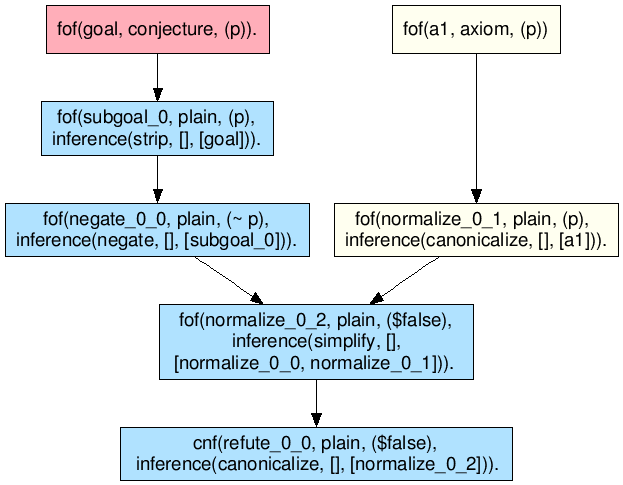
\includegraphics[height=0.8\textwidth]{figures/derivation.png}
     \end{center}
\end{column}
\end{columns}
\vfill
\end{frame}


% \begin{frame}[fragile, label=athena]{\texttt{Athena}~\citep{Athena}}

%  \begin{tikzpicture}[overlay,remember picture]
%  \tikzset{shift={(current page.north)}, xshift=0cm,yshift=0cm}
%   \node[] at (0.92\textwidth, 1cm)
%     {
\includegraphics[width=0.15\textwidth]{figures/athena}};
% \end{tikzpicture}

% Is a \texttt{Haskell} program
% that translates proofs given by \Metis
% in \TSTP format to \texttt{Agda} code\\

% \begin{itemize}
%     \item Parsing of \TSTP language\footnote{\label{parsing}\url{https://github.com/agomezl/tstp2agda}.}
%     \item Creation\textsuperscript{\ref{parsing}} and analysis of \hyperlink{tstp-dag}{\textbf{DAG}} derivations
%     \item Analysis of inference rules used in the \TSTP derivation
%     \item \texttt{Agda} code generation
% \begin{table}[!ht]
% \begin{center}
% \scalebox{0.8}{
% {\renewcommand{\arraystretch}{1.3}%
% \begin{tabular}{|ll| }
% \hline
% \textbf{Library} & \textbf{Purpose} \\
% \hline
% \texttt{\hyperlink{agda-prop}{\texttt{Agda-Prop}}}& axioms and theorems of Classical Propositional Logic\\
% \texttt{\hyperlink{agda-metis}{\texttt{Agda-Metis}}} & versions of the inference rules used by \Metis\\
% \hline
% \end{tabular}}
% }
% \end{center}
% \label{tab:library}
% \end{table}

% \end{itemize}
% \end{frame}

% \begin{frame}[fragile, label=agda-prop-2]{\texttt{Agda-Prop} Library
%   \footnote{\url{https://github.com/jonaprieto/agda-prop}.}}
% \begin{itemize}
%   \item Intuitionistic Propositional Logic + PEM ($\Gamma ⊢ ϕ \vee \neg ϕ$)
%   \item A data type for formulas
%   \vspace*{1mm}

% \begin{minted}{cagda}
% data Prop : Set where
%   Var : Fin n → Prop
%   ⊤   : Prop
%   ⊥   : Prop
%   _∧_ : (\varphi \psi : Prop) → Prop
%   _∨_ : (\varphi \psi : Prop) → Prop
%   _⇒_ : (\varphi \psi : Prop) → Prop
%   _⇔_ : (\varphi \psi : Prop) → Prop
%   ¬_  : (\varphi : Prop)   → Prop
% \end{minted}
% \end{itemize}
% \end{frame}

% \begin{frame}[fragile, label=agda-prop]{\texttt{Agda-Prop} Library~\citep{AgdaProp}}
% \begin{itemize}
%   \item A data type for theorems
%   \vspace*{1mm}
% \begin{minted}{cagda}
% data _⊢_ : (Γ : Ctxt)(\varphi : Prop) → Set
% \end{minted}

% \item Constructors
%   \vspace*{1mm}

% \begin{minted}{cagda}
% assume, axiom, weaken, ⊤-intro, ⊥-elim, ¬-intro,
% ¬-elim, ∧-intro, ∧-proj₁, ∧-proj₂, ∨-intro₁,
% ∨-intro₂, ∨-elim, ⇒-intro, ⇒-elim, ⇔-intro,
% ⇔-elim₁, ⇔-elim₂.
% \end{minted}
%   \item Natural deduction proofs for more than 71 theorems
%   \vspace*{1mm}
% \begin{minted}{cagda}
% ⇔-equiv, ⇔-assoc, ⇔-comm, ⇒-⇔-¬∨, ⇔-¬-to-¬,
% ¬⇔-to-¬, ¬¬-equiv, ⇒⇒-⇔-∧⇒, ⇔-trans, ∧-assoc,
% ∧-comm, ∧-dist, ¬∧-to-¬∨¬, ¬∨¬-to-¬∧, ¬∨¬-⇔-¬∧,
% subst⊢∧₁, subst⊢∧₂, ∨-assoc, ∨-comm, ∨-dist,
% ∨-equiv, ¬∨-to-¬∧¬, ¬∧¬-to-¬∨, ∨-dmorgan,
% ¬¬∨¬¬-to-∨, cnf, nnf, dnf, RAA, ...
% \end{minted}
% \end{itemize}
% \end{frame}


% \begin{frame}[fragile, label=agda-metis]{\texttt{Agda-Metis} Library
%   ~\citep{AgdaMetis}}
% \vfill
% \begin{table}[!ht]
% \begin{center}
% \scalebox{0.7}{
% {\renewcommand{\arraystretch}{1.3}%
% \begin{tabular}{|lll|}
% \hline
% \textbf{Rule} & \textbf{Purpose} &\textbf{Theorem}\\
% \hline
% \texttt{canonicalize} & transforms formulas to CNF, DNF or NNF &\texttt{atp-canonicalize}\\
% \texttt{clausify} & performs clausification &\texttt{atp-clausify}\\
% \hyperlink{atp-conjunct}{\texttt{conjunct}} & takes a formula from a conjunction &\hyperlink{atp-conjunct}{\texttt{atp-conjunct}}\\
% \texttt{negate} & append negation symbol to the formula &\texttt{atp-negate}\\
% \texttt{resolve} & applies theorems of resolution &\texttt{atp-resolve}\\
% \texttt{simplify} & applies over a list of formula to simplify them &\texttt{atp-simplify}\\
% \texttt{strip} & splits a formula into subgoals &\texttt{atp-strip}\\[1ex]
% \hline
% \end{tabular}}
% }
% \end{center}
% \label{tab:agda-metis-table}
% \end{table}
% \vfill
% \end{frame}


% \begin{frame}[fragile, label=atp-conjunct]{\texttt{Agda-Metis}: Conjunct Inference
%   \footnote{\url{https://github.com/jonaprieto/agda-metis}.}
%   }

% \vfill
% \begin{itemize}
% \item Definition
% \begin{equation*}
% \text{\color{blu!40!black}conjunct}(\overbrace{\varphi_1 ∧ ⋯ ∧ \varphi_n}^{\varphi}, \psi)
% = \begin{cases}
% \varphi_{i} \ \ \ \ \text{if }\psi\text{ is equal to some }\varphi_i\\
% \varphi    \ \ \ \ \text{otherwise}
% \end{cases}
% \end{equation*}

% \pause
% \item Inference rules involved
% \begin{center}
% \begin{columns}
% \begin{column}{0.42\textwidth}

%  \begin{prooftree}
%   \AxiomC{$\varphi_1 ∧ \varphi_2$}
%   \RightLabel{\scriptsize $∧$-\texttt{proj}$₁$}
%   \UnaryInfC{$\varphi_1$}
%   \end{prooftree}
% \end{column}

% \begin{column}{0.42\textwidth}
%  \begin{prooftree}
%   \AxiomC{$\varphi_1 ∧ \varphi_2$}
%   \RightLabel{\scriptsize $∧$-\texttt{proj}$₂$}
%   \UnaryInfC{$\varphi₂$}
%   \end{prooftree}
% \end{column}

% \begin{column}{0.2\textwidth}  %%<--- here
%   \begin{tikzpicture}[
%     ->
%   , >=stealth'
%   , shorten >=1pt
%   , auto
% %  , node distance=2.8cm
%   , thick
%   , every state/.style={fill=blu!45!black,draw=none,text=white}
%   , overlay
%   , remember picture
%     , transform canvas={scale=.75}
%     ]
%   \tikzset{shift={(current page.center)}, xshift=4.5cm,yshift=0cm}


%   \node[state]  (phi)                     {$\varphi$};
%   \node[state]  (phi1) [below left =1.3cm and 0.1cm of phi]  {$\varphi_1$};
%   \node[state]  (phi2) [below right=1.3cm and 0.1cm of phi]  {$\varphi_2$};
%   \node[state]  (phi3)  [below left =1.3cm and 0.1cm of phi2]  {$\varphi_3$};
%   \node[state]  (phi4)  [below right =1.3cm and 0.1cm of phi2]  {$\varphi_4$};

%   \path[every node/.style={sloped,anchor=south,auto=false}]
%         (phi) edge node {\tiny $∧$-\texttt{proj}$₁$} (phi1)
%         (phi) edge node {\tiny $∧$-\texttt{proj}$₂$} (phi2)
%         (phi2) edge node {\tiny $∧$-\texttt{proj}$₁$} (phi3)
%         (phi2) edge node {\tiny $∧$-\texttt{proj}$₂$} (phi4);

% \end{tikzpicture}
% \end{column}
% \end{columns}
% \end{center}
% \vskip 2mm

% \item Example
% \[ \varphi := \varphi_1 ∧ \overbrace{(\varphi_3 ∧ \varphi_4)}^{\varphi_2}\]

% \begin{itemize}

% \item
% \texttt{conjunct}$(\varphi , \varphi_3 ∧ \varphi_1) ≡ \varphi$
% \vskip 3mm
% \item
% \texttt{conjunct}$(\varphi , \varphi_3)      ≡ \varphi_3$
% \vskip 3mm
% \item
% \texttt{conjunct}$(\varphi , \varphi_2)      ≡ \varphi_2$
% \vskip 3mm
% \end{itemize}

% \end{itemize}
% \end{frame}

% \begin{frame}[fragile]

% \begin{minted}{cagda}
% data ConjView : Prop → Set where
%   conj  : (\varphi₁ \varphi₂ : Prop) → ConjView (\varphi₁ ∧ \varphi₂)
%   other : (\varphi : Prop)     → ConjView \varphi

% conj-view : (\varphi : Prop) → ConjView \varphi
% conj-view (\varphi ∧ \psi) = conj _ _
% conj-view \varphi       = other _

% data Step : Set where
%   pick  : Step
%   proj₁ : Step
%   proj₂ : Step

% Path : Set
% Path = List Step

% conjunct-path : (\varphi \psi : Prop) → Path → Path
% conjunct-path \varphi \psi path with ⌊ eq \varphi \psi ⌋
% ... | true  = path ∷ʳ pick
% ... | false with conj-view \varphi
% ...   | other _ = []
% ...   | conj \varphi₁ \varphi₂ with conjunct-path \varphi₁ \psi []
% ...     | subpath@(_ ∷ _) = (path ∷ʳ proj₁) ++ subpath
% ...     | [] with conjunct-path \varphi₂ \psi []
% ...          | subpath@(_ ∷ _) = (path ∷ʳ proj₂) ++ subpath
% ...          | []              = []
% \end{minted}

% \end{frame}


% \begin{frame}[fragile, label=atp-conjunct-proof]{The \texttt{conjunct} function and its theorem, \texttt{atp-conjunct}}
% \vfill
% \begin{minted}{cagda}
% conjunct : Prop → Prop → Prop
% conjunct \varphi \psi with conj-view \varphi | conjunct-path \varphi \psi []
% ... | _          | []        = \varphi
% ... | conj _ _   | pick  ∷ _ = \varphi
% ... | conj \varphi₁ _  | proj₁ ∷ _ = conjunct \varphi₁ \psi
% ... | conj _ \varphi₂  | proj₂ ∷ _ = conjunct \varphi₂ \psi
% ... | other .\varphi   | _         = \varphi

% atp-conjunct
%   : ∀ {Γ} {\varphi}
%   → (\psi : Prop)
%   → \Gamma ⊢ \varphi
%   → \Gamma ⊢ conjunct \varphi \psi

% atp-conjunct {Γ} {\varphi} \psi Γ⊢\varphi
%   with conj-view \varphi | conjunct-path \varphi \psi []
% ...  | _           | []        = Γ⊢\varphi
% ...  | conj _ _    | pick  ∷ _ = Γ⊢\varphi
% ...  | conj _ _    | proj₁ ∷ _ = atp-conjunct \psi (∧-proj₁ Γ⊢\varphi)
% ...  | conj _ _    | proj₂ ∷ _ = atp-conjunct \psi (∧-proj₂ Γ⊢\varphi)
% ...  | other _     | (_ ∷ _)   = Γ⊢\varphi
% \end{minted}
% \vfill
% \end{frame}

% \begin{frame}[fragile, label=agda-file]{\texttt{Agda} Code Example}
%   {Generated by \texttt{Athena} Tool}

% \begin{itemize}
%   \item The problem is $p ∧ q ⊢ q ∧ p$
%   \item In \TPTP format
% \begin{tptp}
% $ cat problem.tptp
% fof(a, axiom, p & q).
% fof(goal, conjecture, q & p).
% \end{tptp}
%   \item How to use Athena with your problem

% \begin{tptp}
% $ metis --show proof problem.tptp > problem.tstp
% $ athena problem.tstp
% $ agda problem.tstp
% \end{tptp}
% \end{itemize}
% \end{frame}

% \begin{frame}[fragile, allowframebreaks]{\TSTP Derivation given by \Metis}
% \begin{tptp}
% fof(a, axiom, p & q).
% fof(goal, conjecture, q & p).
% fof(subgoal_0, plain, q,
%     inference(strip, [], [goal])).
% fof(subgoal_1, plain, q => p,
%     inference(strip, [], [goal])).
% fof(negate_0_0, plain, ~ q,
% inference(negate, [], [subgoal_0])).
% fof(normalize_0_0, plain, (~ q),
%     inference(canonicalize, [], [negate_0_0])).
% fof(normalize_0_1, plain, p & q,
%     inference(canonicalize, [], [a])).
% fof(normalize_0_2, plain, q,
%     inference(conjunct, [], [normalize_0_1])).
% fof(normalize_0_3, plain, $false,
%     inference(simplify, [],
%         [normalize_0_0, normalize_0_2])).
% cnf(refute_0_0, plain, $false,
%     inference(canonicalize, [], [normalize_0_3])).
% fof(negate_1_0, plain, ~ (q => p),
%     inference(negate, [], [subgoal_1])).
% fof(normalize_1_0, plain, ~ p & q,
%     inference(canonicalize, [], [negate_1_0])).
% fof(normalize_1_1, plain, p & q,
%      inference(canonicalize, [], [a])).
% fof(normalize_1_2, plain, p,
%     inference(conjunct, [], [normalize_1_1])).
% fof(normalize_1_3, plain, q,
%     inference(conjunct, [], [normalize_1_1])).
% fof(normalize_1_4, plain, $false,
%     inference(simplify, [],
%       [normalize_1_0, normalize_1_2, normalize_1_3])).
% cnf(refute_1_0, plain, ($false),
%     inference(canonicalize, [], [normalize_1_4])).
% \end{tptp}
% \end{frame}

% \begin{frame}[fragile, label=verified-example]{Problem $p ∧ q ⊢ q ∧ p$}{Proof generated with \texttt{Athena}}
% \vfill
% \begin{minted}{cagda}
% p, q, a, goal, subgoal₀, subgoal₁ : Prop

% -- Axiom.
% a = p ∧ q

% -- Premise.
% Γ : Ctxt
% Γ = [ a ]

% -- Conjecture.
% goal = q ∧ p

% -- Subgoals.
% subgoal₀ = q
% subgoal₁ = q ⇒ p
% \end{minted}
% \vfill
% \end{frame}

% \begin{frame}[fragile, label=verified-example-2]{Problem $p ∧ q ⊢ q ∧ p$}{Reconstructed Proof}
% \vfill
% \begin{minted}{cagda}
% a : Prop
% a = p ∧ q

% subgoal₀ : Prop
% subgoal₀ = q

% proof₀ : \Gamma ⊢ subgoal₀
% proof₀ =
%   (RAA
%     (atp-simplify ⊥
%       (assume {Γ = Γ}
%         (\neg subgoal₀))
%       (atp-conjunct q
%         (atp-canonicalize (p ∧ q)
%           (weaken (\neg subgoal₀)
%             (assume {Γ = ∅} a))))))
% \end{minted}
% \vfill
% \end{frame}

% \begin{frame}[fragile, label=verified-example-3]
%   {Problem $p ∧ q ⊢ q ∧ p$}{Reconstructed Proof}
% \vfill
% \begin{minted}{cagda}
% subgoal₁ : Prop
% subgoal₁ = q ⇒ p

% proof₁ : \Gamma ⊢ subgoal₁
% proof₁ =
%   (RAA
%     (atp-simplify ⊥
%       (atp-conjunct q
%         (atp-canonicalize (p ∧ q)
%           (weaken (\neg subgoal₁)
%             (assume {Γ = ∅} a))))
%       (atp-simplify ⊥
%         (atp-canonicalize ((\neg p) ∧ q)
%           (assume {Γ = Γ}
%             (\neg subgoal₁)))
%         (atp-conjunct p
%           (atp-canonicalize (p ∧ q)
%             (weaken (\neg subgoal₁)
%               (assume {Γ = ∅} a)))))))
% \end{minted}
% \vfill
% \end{frame}

% \begin{frame}[fragile, label=verified-example-4]{Problem $p ∧ q ⊢ q ∧ p$}{Reconstructed proof}
% \vfill
% \begin{minted}{cagda}
% -- Premise.
% Γ = [ a ]

% -- Conjecture.
% goal = q ∧ p

% -- Subgoals.
% subgoal₀ = q
% subgoal₁ = q ⇒ p

% -- Proof
% proof₀ : \Gamma ⊢ subgoal₀
% proof₁ : \Gamma ⊢ subgoal₁

% proof : \Gamma ⊢ goal
% proof =
%   ⇒-elim
%     atp-splitGoal            -- q ∧ (q ⇒ p) ⇒ p
%     (∧-intro proof₀ proof₁)
% \end{minted}
% \vfill
% \end{frame}

% \begin{frame}[fragile, label=failure-example]{Bug\footnote{\url{https://github.com/gilith/metis/issues/2}.} in the Printing of the Proof}
%   {\Metis v2.3 (release 20161108)}
% % {}
% \begin{tptp}
% $ cat problem.tptp
% fof(goal, conjecture,
%   ((p <=> q) <=> r) <=> (p <=> (q <=> r))).
% \end{tptp}
% \begin{tptp}
% $ metis --show proof problem.tptp
% ...
% fof(normalize_2_0, plain,
%   (~ p & (~ q <=> ~ r) & (~ p <=> (~ q <=> ~ r))),
%   inference(canonicalize, [], [negate_2_0])).
% fof(normalize_2_1, plain, ~ p <=> (~ q <=> ~ r),
%     inference(conjunct, [], [normalize_2_0])).
% fof(normalize_2_2, plain, ~ q <=> ~ r,
%     inference(conjunct, [], [normalize_2_0])).
% fof(normalize_2_3, plain, ~ p,
%   inference(conjunct, [], [normalize_2_0])).
% fof(normalize_2_4, plain, $false,
%     inference(simplify, [],
%       [normalize_2_1, normalize_2_2, normalize_2_3])).
% ...
% \end{tptp}
% \end{frame}

% \begin{frame}[fragile, label=failure-example-2]{Bug in the Printing of the Proof}
%   {\Metis v2.3 (release 20161108)}

% \[ \varphi := \neg p ∧ (\neg q ⇔ \neg r) ∧ (\neg p ⇔ (\neg q ⇔ \neg r))\]

% \begin{prooftree}
% \AxiomC{$\vdots$}
% \RightLabel{\scriptsize{canonicalize}}
% \UnaryInfC{$\varphi$}
% \RightLabel{\scriptsize{conjunct}}
% \UnaryInfC{$\neg p ⇔ (\neg q ⇔ \neg r)$}

% \AxiomC{$\vdots$}
% \RightLabel{\scriptsize{canonicalize}}
% \UnaryInfC{$\varphi$}
% \RightLabel{\scriptsize{conjunct}}
% \UnaryInfC{$\neg q ⇔ \neg r$}

% \AxiomC{$\vdots$}
% \RightLabel{\scriptsize{canonicalize}}
% \UnaryInfC{$\varphi$}
% \RightLabel{\scriptsize{conjunct}}
% \UnaryInfC{$\neg p$}

% \RightLabel{\scriptsize{simplify}}
% \TrinaryInfC{$\bot$}
% \end{prooftree}
% \pause
% The bug was caused by the conversion of \texttt{Xor} sets to \texttt{Iff} lists.
% After reporting this, Hurd fixed the printing of \texttt{canonicalize} inference rule
% \[ \varphi := \neg p ∧ (\neg q ⇔ \neg r) ∧ (\neg p ⇔ (\neg q ⇔ {\color{red} r}))\]
% \end{frame}


% \begin{frame}[fragile, label=hammer]{Related Work}
% \begin{block}{SledgeHammer} \citep{Paulson2007}
% \begin{itemize}
% \item \texttt{Isabelle}/\texttt{HOL} mature tool
% \item \Metis ported within \texttt{Isabelle/HOL}
% \item Reconstruct proofs of well-known ATPs: \texttt{EProver}, \texttt{Vampire},
% among others using \texttt{SystemOnTPTP} server
% \end{itemize}
% \end{block}

% \begin{block}{Integrating \texttt{Waldmeister} into \texttt{Agda}} \citep{Foster2011}
% \begin{itemize}
%   \item Framework for a integration between \texttt{Agda} and ATPs
%   \begin{itemize}
%     \item Equational Logic
%     \item Reflection Layers
%   \end{itemize}
%   \item Source code is not available\footnote{\url{http://simon-foster.staff.shef.ac.uk/agdaatp}.}
%   \end{itemize}
% \end{block}
% \end{frame}



% \begin{frame}[fragile]{Related Work: \texttt{Apia}}
%   {Proving First-Order theorems written in \texttt{Agda} using automatic
%   theorem provers for First-Order Logic}

% \only<1>{At the moment, the communication between \texttt{Agda} and
% the ATPs is unidirectional because the ATPs are being used as oracles \citep{Sicard2015}
% \vfill
% }
% \only<1>{
% \inputminted{cagda}{Or.agda}
% \begin{tikzpicture}[overlay, remember picture, scale=0.5]
% \tikzset{shift={(current page.center)}, xshift=6cm,yshift=-2cm}
% \node(agdafile) at (0,0){
%   
\includegraphics[scale=0.8]{figures/agda-pragmas}};
% \end{tikzpicture}
% }

% \begin{tikzpicture}

% \only<2->{ \node(agdafile) at (0,0){
%   
\includegraphics[scale=0.8]{figures/agda-pragmas}}};

% \only<2->{
%   \node[right=1cm of agdafile] (eagda){
%   
\includegraphics[scale=0.8]{figures/eagda}
%   \footnote{\url{https://github.com/asr/eagda}.}
%   }
% };

% \only<2->{
% \node[right=1cm of eagda] (agdai){
%   
\includegraphics[scale=0.8]{figures/agdai}
%   }
% };

% \only<3->{
%   \node[below=0.4cm of agdai] (apia){
%   
\includegraphics[scale=0.8]{figures/apia}
%   \footnote{\url{https://github.com/asr/apia}.}}
%   };

% \only<4->{
%   \node[below= 0.4cm of eagda] (tptp)
%     {
\includegraphics[scale=0.8]{figures/tptp}}};

% \only<5->{ \node[below = 0.8cm of apia] (atp)
%   {
\includegraphics[scale=0.8]{figures/atp}
%   \footnote{\url{http://github.com/jonaprieto/online-atps}.}}
%   };

% \only<7->{ \node[left= 2cm of atp, rectangle, text=white,fill=black, align=left, font=\small] (proved)
% {
% \texttt{\$ agda Or.agda}\\
% \texttt{\$ apia Or.agda --atp=online-metis}\\
% \texttt{Metis---2.3 proved the conjecture}
%   }
% };

% \only<2->{\draw[->, ultra thick] (agdafile) to (eagda)};
% \only<2->{\draw[->, ultra thick] (eagda) to (agdai)};
% \only<3->{\draw[->, ultra thick] (agdai) to (apia)};
% \only<4->{\draw[->, very thick, dashed, gray] (apia) to (tptp)};
% \only<5->{\draw[->, very thick, dashed, gray] (tptp) to (atp)};
% \only<6->{\draw[->, very thick, dashed, gray] (atp) to (apia)};
% \end{tikzpicture}
% \end{frame}


% \begin{frame}[fragile,label=metis-inference-rules]{\Metis Inference Rules}
% \vfill
% \begin{prooftree}
% \AxiomC{}
% \RightLabel{axiom}
% \UnaryInfC{$C$}
% \end{prooftree}
% \vfill
% \begin{prooftree}
% \AxiomC{}
% \RightLabel{assume $L$}
% \UnaryInfC{$L \vee \neg L$}
% \end{prooftree}
% \vfill
% \begin{prooftree}
% \AxiomC{$C$}
% \RightLabel{subst $σ$}
% \UnaryInfC{$σC$}
% \end{prooftree}
% \vfill
% \begin{prooftree}
% \AxiomC{$L \vee C$}
% \AxiomC{$\neg L \vee D$}
% \RightLabel{resolve $L$}
% \BinaryInfC{$C \vee D$}
% \end{prooftree}
% \vfill
% \begin{prooftree}
% \AxiomC{}
% \RightLabel{refl $t$}
% \UnaryInfC{$t = t$}
% \end{prooftree}
% \vfill
% \begin{prooftree}
% \AxiomC{}
% \RightLabel{eq $L$ $p$ $t$}
% \UnaryInfC{$\neg (L[p] = t) \vee \neg L \vee L[ p ↦ t]$}
% \end{prooftree}
% \vfill
%  \begin{tikzpicture}[overlay, remember picture, scale=0.5]
%     \tikzset{shift={(current page.center)}, xshift=11.8cm,yshift=-8.4cm}
%     \node[fill=blu,text=white, hyperlink node = metis]
%       (go) at (0,0) {\tiny Go Back};
%   \end{tikzpicture}
% \end{frame}
\end{document}
